\documentclass[12pt]{article}
\usepackage[margin=1in]{geometry}
\usepackage{setspace}
\usepackage{booktabs}
\usepackage{threeparttable}
\usepackage{tikz}
\usetikzlibrary{positioning,arrows.meta}
\usepackage{fancyhdr}
\usepackage{natbib}
\usepackage[hidelinks]{hyperref}

\pagestyle{fancy}
\fancyhf{}
\fancyhead[L]{\small SYNTHETIC TEST PAPER, NOT REAL RESEARCH}
\fancyhead[R]{\small Psychological safety and managerial voice}
\fancyfoot[C]{\thepage}
\renewcommand{\headrulewidth}{0.4pt}

\onehalfspacing

\begin{document}

\thispagestyle{empty}
\begin{center}
\vspace*{0.5in}
{\large\textbf{SYNTHETIC TEST PAPER, NOT REAL RESEARCH}}\\[0.3in]
{\small This paper was written to test a reviewing tool. The country, panel vendor, respondents, authors, and cited scales are fictional. Only the methods papers in the reference list are real.}\\[0.8in]
{\LARGE\textbf{Speaking Up Because It Is Safe:\\[0.1in] Psychological Safety, Felt Obligation, and Managerial Voice}}\\[0.6in]
{\large Mira Tallsen}\\
Veloria School of Business, Port Averin, Veloria\\[0.2in]
{\large Joren Okafor-Vay}\\
Institute for Work and Organization, University of Ostmere, Veloria\\[0.8in]
Draft prepared for submission, 2024
\end{center}
\clearpage\setcounter{page}{2}

\begin{abstract}
\noindent Managers often hold information that senior leaders need but do not hear. We argue that psychological safety increases voice because managers who feel safe come to feel obligated to improve their unit. Using a questionnaire completed by 402 managers from an online panel in Veloria, we fit a path model to the correlations among psychological safety, felt obligation, voice, and two controls. Psychological safety increases voice both directly and through felt obligation, and the indirect path is significant. The findings identify felt obligation as the mechanism that links a safe climate to speaking up and show that organizations can raise managerial voice by investing in psychological safety.

\medskip
\noindent\textit{Keywords:} psychological safety; voice; felt obligation; middle managers; path model
\end{abstract}

\section{Introduction}

Organizations depend on managers to raise problems and suggestions before those problems become expensive. Middle managers see operational failures early, they translate strategy into routines, and they are often the first to notice when a plan no longer fits the conditions it was built for. Yet a large share of what managers know never travels upward. Managers stay silent when they expect speaking up to be costly to their standing, when they doubt that anyone will act on what they say, or when they see voice as someone else's job.

A line of work in Veloria and elsewhere treats psychological safety, the shared belief that a work group is safe for interpersonal risk taking, as a precondition for voice \citep{dravenko2015}. When people believe that a mistake or a challenge will not be held against them, the expected cost of voice falls. Most of this work, however, studies frontline employees. Managers occupy a different position. They supervise others, they are evaluated on the performance of their unit, and their voice is directed at senior leaders whose decisions shape their careers. Whether psychological safety matters in the same way for them is an open question.

This paper makes two arguments. First, psychological safety increases the voice of managers. Second, it does so in part because it raises managers' felt obligation, the sense that they are responsible for improving their unit and the organization. A manager who feels safe is more likely to see problems as things she is expected to fix and less likely to see them as risks to avoid. Felt obligation then turns that sense of responsibility into speaking up.

Our central contribution is an estimate of the causal effect of psychological safety on managerial voice and of the share of that effect that runs through felt obligation. We study 402 managers who completed an online questionnaire in March 2024, and we fit a path model to the correlations among the study variables. The results show a large effect of psychological safety on voice and a smaller but reliable indirect path through felt obligation. For practice, the results point to a lever that senior leaders control: the climate in which managers work.

\section{Theory and Hypotheses}

\subsection{Psychological safety and voice}

Voice is discretionary communication of ideas, suggestions, concerns, or opinions intended to improve how a unit works \citep{pell2018}. Because voice challenges the status quo, it carries risk. The person who speaks up may be seen as disloyal, uninformed, or difficult, and the costs fall on the speaker while the gains are shared. People weigh these costs before they speak.

Psychological safety changes this calculation. In a psychologically safe group, members expect that others will not embarrass, reject, or punish someone for speaking up \citep{dravenko2015}. The expected cost of voice falls, and so voice rises. For managers, the relevant group is the set of peers and superiors with whom they work most closely. A manager who expects that a candid concern will be received as a contribution, and not as a sign of weakness, has less reason to stay quiet.

\medskip
\noindent\textit{Hypothesis 1.} Psychological safety increases managerial voice.

\subsection{The role of felt obligation}

Felt obligation is a belief that one ought to care about the well-being of the organization and help it reach its goals \citep{quennell2016}. Felt obligation grows when people see their environment as supportive and fair. A psychologically safe climate signals that the organization values members' contributions and will treat them well when they take risks on its behalf. Managers who receive that signal reciprocate with a stronger sense that improving the unit is their responsibility.

Felt obligation, in turn, is a reason to speak up. A manager who believes she is responsible for the unit's performance will see silence about a known problem as a failure of that responsibility. Voice becomes a way to discharge a duty. We therefore expect felt obligation to carry part of the effect of psychological safety on voice. We do not expect it to carry the whole effect, because psychological safety also lowers the perceived cost of voice directly.

\medskip
\noindent\textit{Hypothesis 2.} Felt obligation mediates the positive effect of psychological safety on managerial voice.

\section{Method}

\subsection{Sample and procedure}

We collected data through Ardent Insight, an opt-in online research panel that operates in Veloria and recruits adults who agree to complete paid questionnaires. The questionnaire was fielded between 4 and 22 March 2024. Ardent Insight invited panel members whose profiles listed full-time employment. Respondents qualified for the study by indicating in a screening question that they currently held a managerial position with at least one direct report. Respondents who did not select this option were routed out of the questionnaire before the main items.

The questionnaire included one attention check item, embedded in the voice scale, that asked respondents to select ``somewhat disagree.'' \citet{meade2012} show that careless responding can distort the correlations among survey scales. Respondents who failed the attention check were removed, leaving a final sample of 402 managers. Respondents received the panel's standard incentive, which is paid in points redeemable for vouchers.

Of the 402 managers, 57.2 percent were men and 42.8 percent women. Their mean age was 41.6 years (SD = 9.2). They worked in manufacturing (22.4 percent), retail and hospitality (18.9 percent), professional services (17.2 percent), health and social care (14.7 percent), public administration (11.9 percent), and other sectors (14.9 percent). The median number of direct reports was six. On average, respondents had been with their current organization for 6.83 years (SD = 5.21).

\subsection{Measures}

All variables were measured in the same online questionnaire, which each respondent completed in a single session. Unless noted, items used a seven-point response scale from 1 (strongly disagree) to 7 (strongly agree), and scale scores are the mean of the items. Following \citet{flake2020}, we report every item in Appendix A. No items were changed from the published versions.

\textit{Psychological safety.} We used the seven-item scale of \citet{dravenko2015}, with the work group defined for respondents as ``the peers and senior managers you work with most closely.'' A sample item is ``In this group, I can raise a problem without worrying about how it will reflect on me.'' Cronbach's alpha was .88. We treat psychological safety as each manager's own perception of this group and analyze it at the individual level; we make no claim about a climate shared by the group's members.

\textit{Voice.} We used the six-item managerial voice scale of \citet{pell2018}. Respondents reported how often in the past three months they had engaged in each behavior toward senior leaders, on a scale from 1 (never) to 7 (always). A sample item is ``I spoke up with ideas for new projects or changes in procedures.'' Cronbach's alpha was .90.

\textit{Felt obligation.} We used the five-item scale of \citet{quennell2016}. A sample item is ``I feel a personal obligation to do whatever I can to help my unit improve.'' Cronbach's alpha was .84.

\textit{Team trust.} To separate psychological safety from trust in one's closest colleagues, a related but distinct construct, we measured team trust with the five-item scale of \citet{olumide2017}. A sample item is ``I can rely on the people I work with most closely to follow through on their commitments.'' Cronbach's alpha was .86.

\textit{Controls.} We controlled for two variables. Organizational tenure, in years, captures the standing that longer-serving managers may have to raise issues, which could raise both felt obligation and voice; respondents reported it directly. Prosocial motivation, the desire to benefit others through one's work, is a relatively stable disposition that could make a manager more likely both to feel obligated and to speak up \citep{tesfaye2014}. We measured it with four items (alpha = .83). We report every model with and without the controls.

\subsection{Measurement model}

We estimated a confirmatory factor analysis of the five multi-item scales (27 items) with maximum likelihood. The five-factor model fit the data well, $\chi^2(314) = 604.3$, CFI = .96, TLI = .95, RMSEA = .048, SRMR = .041, against the cutoffs of .95 for CFI and TLI, .06 for RMSEA, and .08 for SRMR proposed by \citet{hu1999}. All standardized loadings were between .64 and .87.

Psychological safety and team trust are strongly correlated (Table 1). To test whether respondents distinguished them, we compared the five-factor model with a four-factor model in which the psychological safety and team trust items loaded on one factor. The four-factor model fit markedly worse, $\chi^2(318) = 1{,}187.6$, CFI = .88, RMSEA = .083, SRMR = .069; $\Delta\chi^2(4) = 583.3$, $p < .001$. We therefore treat the two as distinct constructs.

\subsection{Analysis}

We tested the hypotheses with the path model in Figure 1. Psychological safety predicts felt obligation, and both predict voice. In Model 2 the two controls predict both felt obligation and voice. We fitted the model to the correlation matrix in Table 1 by maximum likelihood with N = 402, so all coefficients are standardized. Both models are saturated, so their fit is perfect by construction and we do not report fit indices for them. Following \citet{zhao2010}, we tested mediation with the indirect effect itself, the product of the path from psychological safety to felt obligation and the path from felt obligation to voice. We formed a 95 percent Monte Carlo confidence interval for the indirect effect from 20,000 draws of the two path estimates.

\section{Results}

Table 1 reports means, standard deviations, and correlations. Psychological safety is strongly correlated with voice (r = .74) and moderately correlated with felt obligation (r = .50). Felt obligation is correlated with voice (r = .53).

\begin{table}[p]
\centering
\begin{threeparttable}
\caption{Means, standard deviations, and correlations}
\label{tab:corr}
\begin{tabular}{lcccccccc}
\toprule
Variable & Mean & SD & 1 & 2 & 3 & 4 & 5 & 6 \\
\midrule
1. Psychological safety & 5.12 & 1.03 &  &  &  &  &  &  \\
2. Team trust & 5.34 & 0.98 & .79 &  &  &  &  &  \\
3. Voice & 4.87 & 1.14 & .74 & .05 &  &  &  &  \\
4. Felt obligation & 5.41 & 0.92 & .50 & .47 & .53 &  &  &  \\
5. Prosocial motivation & 5.76 & 0.84 & .38 & .34 & .41 & .44 &  &  \\
6. Tenure & 6.83 & 5.21 & .07 & .04 & .10 & .03 & .06 &  \\
\bottomrule
\end{tabular}
\begin{tablenotes}\footnotesize
\item \textit{Note.} N = 402. The diagonal is left blank; reliabilities are reported in the text. Correlations of .10 or larger in absolute value are significant at p $<$ .05 (two-tailed). Variables 1 to 5 are scored on seven-point scales; tenure is in years.
\end{tablenotes}
\end{threeparttable}
\end{table}

Table 2 reports the path model without controls (Model 1) and with controls (Model 2). Figure 1 shows the estimates from Model 2. Hypothesis 1 predicted that psychological safety increases voice. In Model 2 the direct path from psychological safety to voice is large and significant ($\beta = .61$, SE = .04, $p < .01$), and it is nearly the same size in Model 1 ($\beta = .63$, SE = .04, $p < .01$). Hypothesis 1 is supported.

Hypothesis 2 predicted that felt obligation mediates the effect. Psychological safety increases felt obligation ($\beta = .39$, SE = .04, $p < .01$), and felt obligation increases voice ($\beta = .18$, SE = .04, $p < .01$). The indirect effect is .07, with a 95 percent confidence interval from .04 to .11 that excludes zero. In Model 1 the indirect effect is .11 [.07, .15]. Because the direct path remains significant, felt obligation partially mediates the effect of psychological safety on voice. Hypothesis 2 is supported. The model explains 59 percent of the variance in voice.

\begin{table}[p]
\centering
\begin{threeparttable}
\caption{Path model estimates}
\label{tab:path}
\begin{tabular}{lcccc}
\toprule
 & \multicolumn{2}{c}{Model 1} & \multicolumn{2}{c}{Model 2} \\
\cmidrule(lr){2-3}\cmidrule(lr){4-5}
 & Felt obligation & Voice & Felt obligation & Voice \\
\midrule
Psychological safety & .50*** & .63*** & .39*** & .61*** \\
 & (.04) & (.04) & (.04) & (.04) \\
Felt obligation &  & .21*** &  & .18*** \\
 &  & (.04) &  & (.04) \\
Tenure &  &  & $-$.01 & .05 \\
 &  &  & (.04) & (.03) \\
Prosocial motivation &  &  & .29*** & .10*** \\
 &  &  & (.04) & (.04) \\
\midrule
R$^2$ & .25 & .58 & .32 & .59 \\
\midrule
Indirect effect via felt obligation & \multicolumn{2}{c}{.11 [.07, .15]} & \multicolumn{2}{c}{.07 [.04, .11]} \\
\bottomrule
\end{tabular}
\begin{tablenotes}\footnotesize
\item \textit{Note.} N = 402. Standardized coefficients from a path model fitted to the correlation matrix in Table 1 by maximum likelihood. Standard errors in parentheses. The indirect effect is reported with a 95 percent Monte Carlo confidence interval (20,000 draws). Both models are saturated. *** p $<$ .01, ** p $<$ .05, * p $<$ .10.
\end{tablenotes}
\end{threeparttable}
\end{table}

\begin{figure}[!htbp]
\centering
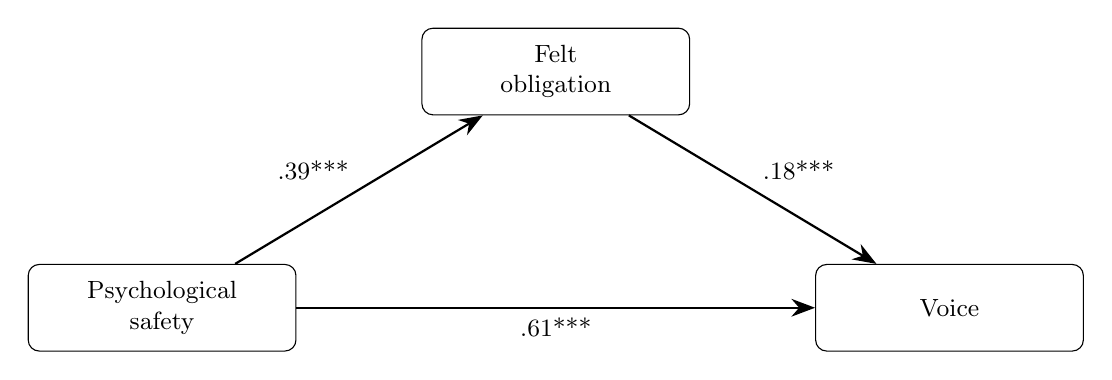
\begin{tikzpicture}[
  box/.style={draw, rounded corners, minimum width=3.4cm, minimum height=1.1cm, align=center, font=\small},
  arr/.style={-{Stealth[length=3mm]}, thick}]
\node[box] (ps) at (0,0) {Psychological\\safety};
\node[box] (fo) at (5,3) {Felt\\obligation};
\node[box] (v) at (10,0) {Voice};
\draw[arr] (ps) -- node[above left, font=\small] {.39***} (fo);
\draw[arr] (fo) -- node[above right, font=\small] {.18***} (v);
\draw[arr] (ps) -- node[below, font=\small] {.61***} (v);
\end{tikzpicture}
\caption{Path model of psychological safety, felt obligation, and voice (Model 2). Standardized coefficients; tenure and prosocial motivation are controlled but not shown. Indirect effect = .07, 95 percent CI [.04, .11]. *** p $<$ .01.}
\label{fig:path}
\end{figure}

\section{Discussion}

We set out to explain why some managers speak up to senior leaders while others stay silent. The answer our data give is that psychological safety increases voice, and that part of this effect runs through a stronger sense of felt obligation. Managers who feel safe with their peers and superiors come to see the unit's problems as theirs to solve, and they speak up more as a result.

\subsection{Theoretical contributions}

The study adds to research on voice in three ways. First, it moves the study of psychological safety from frontline employees to managers. The effect we estimate for managers is large. A one standard deviation increase in psychological safety raises voice by more than six tenths of a standard deviation through the direct path alone. Managers are thus at least as responsive to climate as the employees who have been the focus of past work.

Second, the study identifies felt obligation as a mechanism. Prior accounts explain the link between psychological safety and voice mostly through lower expected costs. Our results show that psychological safety also works through a sense of duty. The indirect path is smaller than the direct path, which fits our argument that safety both lowers costs and raises obligation.

Third, by separating psychological safety from team trust in the measurement model, the study shows that the effect on voice belongs to the climate for interpersonal risk and not to trust in colleagues' reliability. The two constructs are strongly related, but respondents clearly distinguished them.

\subsection{Practical implications}

The results have direct implications for senior leaders. Because psychological safety increases voice, managers should build psychological safety to raise voice in their own teams, and senior leaders should build it among the managers who report to them. Leaders can do this by responding to bad news with questions instead of blame, by acknowledging their own mistakes, and by rewarding managers who raise problems early. Organizations that want more upward information from their managers should treat psychological safety as an investment with a measurable return in voice. Our estimates suggest that the return is large.

Organizations can also raise voice by strengthening felt obligation. Programs that give managers visible ownership of their unit's results, and that connect those results to the organization's goals, should increase the share of managers who see speaking up as part of their job.

\subsection{Limitations and future research}

Our data are cross-sectional, so future research should replicate these findings with longitudinal data. The study was also conducted in a single country. Veloria has relatively low power distance by regional standards, and the effect of psychological safety on managerial voice may be weaker where hierarchies are steeper. Future research could also examine whether felt obligation matters more for some forms of voice, such as raising concerns, than for others, such as proposing new ideas.

\section{Conclusion}

Managers who feel psychologically safe speak up more, and they do so partly because safety makes them feel responsible for their unit. Organizations that want to hear from their managers have a clear place to start.

\begin{thebibliography}{99}
\setlength{\itemsep}{2pt}

\bibitem[Dravenko and Pell(2015)]{dravenko2015}
Dravenko, A., \& Pell, T. (2015). Safe to speak: Developing a measure of psychological safety in work groups. \textit{Veloria Journal of Organizational Studies}, 12(2), 88--107. [Fictional source.]

\bibitem[Flake and Fried(2020)]{flake2020}
Flake, J. K., \& Fried, E. I. (2020). Measurement schmeasurement: Questionable measurement practices and how to avoid them. \textit{Advances in Methods and Practices in Psychological Science}, 3(4), 456--465.

\bibitem[Hu and Bentler(1999)]{hu1999}
Hu, L., \& Bentler, P. M. (1999). Cutoff criteria for fit indexes in covariance structure analysis: Conventional criteria versus new alternatives. \textit{Structural Equation Modeling}, 6(1), 1--55.

\bibitem[Meade and Craig(2012)]{meade2012}
Meade, A. W., \& Craig, S. B. (2012). Identifying careless responses in survey data. \textit{Psychological Methods}, 17(3), 437--455.

\bibitem[Olumide-Carrow(2017)]{olumide2017}
Olumide-Carrow, S. (2017). Trust among close colleagues: Scale development and validation. \textit{Veloria Journal of Organizational Studies}, 14(1), 23--41. [Fictional source.]

\bibitem[Pell et al.(2018)]{pell2018}
Pell, T., Sarrazine, M., \& Oduya, K. (2018). Upward voice among managers: A six-item measure. \textit{Ostmere Review of Management}, 9(3), 201--219. [Fictional source.]

\bibitem[Quennell and Barros-Idde(2016)]{quennell2016}
Quennell, R., \& Barros-Idde, L. (2016). Felt obligation toward the work unit: Construct and measure. \textit{Ostmere Review of Management}, 7(4), 310--328. [Fictional source.]

\bibitem[Tesfaye-Morrow(2014)]{tesfaye2014}
Tesfaye-Morrow, H. (2014). Prosocial motivation at work: A short form. \textit{Veloria Journal of Organizational Studies}, 11(3), 150--166. [Fictional source.]

\bibitem[Zhao et al.(2010)]{zhao2010}
Zhao, X., Lynch, J. G., \& Chen, Q. (2010). Reconsidering Baron and Kenny: Myths and truths about mediation analysis. \textit{Journal of Consumer Research}, 37(2), 197--206.

\end{thebibliography}

\clearpage
\appendix
\section*{Appendix A. Items}

All items used a seven-point scale from 1 (strongly disagree) to 7 (strongly agree), except voice, which used a seven-point frequency scale from 1 (never) to 7 (always). The work group was defined for respondents as ``the peers and senior managers you work with most closely.''

\medskip
\noindent\textbf{Psychological safety} \citep{dravenko2015}
\begin{enumerate}\setlength{\itemsep}{0pt}
\item In this group, I can raise a problem without worrying about how it will reflect on me.
\item If I make a mistake in this group, it is not held against me.
\item Members of this group are able to bring up tough issues.
\item It is safe to take a risk in this group.
\item No one in this group would deliberately act in a way that undermines my efforts.
\item It is easy to ask other members of this group for help.
\item My skills and talents are valued and used in this group.
\end{enumerate}

\noindent\textbf{Voice} \citep{pell2018}. In the past three months, how often have you:
\begin{enumerate}\setlength{\itemsep}{0pt}
\item Spoken up with ideas for new projects or changes in procedures.
\item Raised concerns about problems in how work is done.
\item Told senior leaders about issues that could hurt performance.
\item Made suggestions to improve your unit's results.
\item Spoken up about practices you thought were unwise, even when others disagreed.
\item Proposed solutions to problems you had noticed.
\end{enumerate}

\noindent\textbf{Felt obligation} \citep{quennell2016}
\begin{enumerate}\setlength{\itemsep}{0pt}
\item I feel a personal obligation to do whatever I can to help my unit improve.
\item I owe it to my organization to give my best effort.
\item I have an obligation to help my unit reach its goals.
\item I would feel guilty if I did not raise a problem I knew about.
\item Improving how my unit works is part of my responsibility.
\end{enumerate}

\noindent\textbf{Team trust} \citep{olumide2017}
\begin{enumerate}\setlength{\itemsep}{0pt}
\item I can rely on the people I work with most closely to follow through on their commitments.
\item The people I work with most closely are competent at their jobs.
\item I can count on my closest colleagues to do what they say.
\item My closest colleagues keep the promises they make.
\item I am confident in the abilities of the people I work with most closely.
\end{enumerate}

\noindent\textbf{Prosocial motivation} \citep{tesfaye2014}
\begin{enumerate}\setlength{\itemsep}{0pt}
\item I care about benefiting others through my work.
\item I want to help others through my work.
\item It is important to me to have a positive effect on others through my work.
\item I do my work because I want to make a difference to other people.
\end{enumerate}

\end{document}
